\chapter{Quick start with example A}\label{uch:quick}\label{ch:c7}
This chapter runs the first coupled model: example~A, \cmd{examples/Liard\_groundwater}, in which Raven builds the
groundwater model. It shows every line added to an ordinary Raven model. The same steps, with more explanation, are
Workshop~1.

\begin{plain}
This chapter walks through a real example --- the Liard River in northern Canada --- from input files to results.
Chapter~\ref{uch:build} then shows how to set up your own watershed.
\end{plain}

\section{Install Raven and the MODFLOW~6 library}\label{sec:uinstall}
\begin{enumerate}
\item Get Raven with the coupling (RavenHydroFramework). The coupling is offered to the Raven team for inclusion; until it
is part of Raven, use the \cmd{mf6-coupling} branch of \url{https://github.com/rarabzad/RavenHydroFramework}. Beside it,
get RavenHydroFramework-extra (branch \cmd{main} of \url{https://github.com/rarabzad/RavenHydroFramework-extra};
Reference, Section~\ref{R-sec:building}).
\item Build Raven with CMake: \cmd{cmake -S . -B build}, then \cmd{cmake --build build --config Release} (an optimised
\cmd{Release} build by default).
\item The same build gets the MODFLOW~6 library. With a Fortran compiler, meson~$\geq$~1.7, ninja and git, and the
MODFLOW~6 repository reachable, it builds the library from source. Otherwise (also offline) it downloads the official
release library (Linux x86\_64, Windows x64, Apple Silicon Macs). Either way the library ends up next to Raven, which
finds it without any setting (Reference, Section~\ref{R-sec:building}).
\item If Raven was built without the library (\cmd{make} in \cmd{src/}, \cmd{src/Raven.sln}, \cmd{-DRAVEN\_MF6=OFF}, or
the configure warned that it found no way to get it), get it with \cmd{python tools/get\_mf6.py} in the
RavenHydroFramework-extra repository (Reference, Section~\ref{R-sec:getmf6}). The coupling needs MODFLOW~6.5 or newer; it
was tested with 6.8.1 and 6.6.3, and 6.8 or newer is recommended.
\item \cmd{get\_mf6.py} has no library for Linux other than x86\_64 (e.g.\ aarch64), for Windows on ARM64, or for Intel
Macs (only with \cmd{--version 6.6.3}). There, build the library with Raven: \cmd{cmake -S . -B build -DRAVEN\_MF6=SOURCE},
or give a library you have with \cmd{-DRAVEN\_MF6=PATH -DRAVEN\_MF6\_PATH=/path/to/libmf6.so}.
\end{enumerate}
\begin{inpractice}
\cmd{examples/README.md} gives these steps command by command for Windows, Linux and macOS. The release package for
Linux has Raven and the library ready in its \cmd{bin/} folder.
\end{inpractice}

\section{The example}\label{ch:tutorial}
Example~A is the Liard River model (65 subbasins, 1\,107 HRUs, northern British Columbia and Yukon) with an aquifer
added under three nested subbasins (52, 48 and 43; about 13\,800 km$^2$, 85 coupled HRUs). The other 62 subbasins run
exactly as they do without groundwater.

The original Liard package was made for Raven 2.9.1. For Raven 4.x its Windows paths use \texttt{/}, and the parameter
\cmd{DEP\_THRESHHOLD} is spelled \cmd{DEP\_THRESHOLD}. The example files already include these changes.

Four of Raven's files change. The next four sections show what was added to each.

\section{Step 1: mark the HRUs with groundwater (.rvh)}
In the \cmd{:HRUs} table, the \cmd{AQUIFER\_PROFILE} column was filled for the HRUs of subbasins 52, 48 and 43:
\cmd{VALLEY\_ALLUVIUM} for forest, shrub and wetland HRUs; \cmd{UPLAND\_TILL} for barren HRUs. Glaciers keep
\cmd{[NONE]}. A group listing the same HRUs was added at the end of the file:
\par\noindent\begin{minipage}{\linewidth}
\begin{lstlisting}
:HRUGroup AquiferHRUs
  2736, 2745, 2747, ...
:EndHRUGroup
\end{lstlisting}
\end{minipage}\par\smallskip

\section{Step 2: describe the aquifer (.rvp)}
Added at the end of \cmd{Liard.rvp}:
\begin{lstlisting}
:AquiferClasses
  :Attributes, K_HORIZ, K_VERT, SPEC_STORAGE, SPEC_YIELD, POROSITY
  :Units,      m/d,     m/d,    1/m,          none,       none
  GRAVEL,      50.0,    5.0,    1.0E-5,       0.25,       0.30
  CLAY_TILL,   0.001,   0.0001, 1.0E-4,       0.03,       0.40
  SAND,        10.0,    1.0,    1.0E-5,       0.20,       0.35
  UPLAND_TILL, 0.2,     0.02,   1.0E-4,       0.08,       0.30
:EndAquiferClasses

:AquiferProfiles
  VALLEY_ALLUVIUM, 3, GRAVEL, 15.0, AQUIFER, CLAY_TILL, 5.0, AQUITARD, SAND, TO_BEDROCK, CONFINED_AQUIFER
  UPLAND_TILL,     1, UPLAND_TILL, TO_BEDROCK, AQUIFER
:EndAquiferProfiles

:AquiferProfileParameters
  :Attributes,     INITIAL_HEAD_DEPTH, DEFAULT_BEDROCK_DEPTH, SEEPAGE_LEAKANCE, SOIL_ZONE_DEPTH
  :Units,          m,                  m,                     1/d,              m
  VALLEY_ALLUVIUM, 3.0,                60.0,                  1.0,              0.0
  UPLAND_TILL,     8.0,                15.0,                  1.0,              0.0
:EndAquiferProfileParameters
\end{lstlisting}
The valley aquifer is a gravel layer (15 m) over a clay-till aquitard (5 m) over sand down to bedrock. The uplands have
one till layer down to shallow bedrock. Section~\ref{sec:uprofiles} explains each block.

\section{Step 3: switch the coupling on and send recharge to it (.rvi)}
\par\noindent\begin{minipage}{\linewidth}
\begin{lstlisting}
:GroundwaterModel MODFLOW6
:DefineHRUGroups AquiferHRUs
...
:Percolation PERC_CONSTANT FAST_RESERVOIR SLOW_RESERVOIR
  :-->Conditional HRU_GROUP IS_NOT AquiferHRUs     # existing process, only for uncoupled HRUs
:Percolation PERC_CONSTANT FAST_RESERVOIR GROUNDWATER
  :-->Conditional HRU_GROUP IS AquiferHRUs         # new: this water becomes recharge
\end{lstlisting}
\end{minipage}\par\smallskip
Seepage returns to the lowest soil layer (\cmd{SLOW\_RESERVOIR}), whose existing baseflow process carries it to the
rivers. Aquifer--river exchange goes directly to the reaches.

\section{Step 4: the groundwater file (.rvg)}
\begin{lstlisting}
#########################################################################
# Liard.rvg - Raven-MODFLOW 6 groundwater file (Liard River test case)
#   Groundwater under Central Liard subbasins 52 -> 48 -> 43 (85 HRUs).
#   Hydrogeology (aquifer classes, profiles) is in Liard.rvp;
#   which HRUs have groundwater is set by AQUIFER_PROFILE in Liard.rvh.
#########################################################################

# --- geometry (stand-in data built by tools_build_standin_inputs.py; replace with real data) ---
:HRUGeometry        Liard_HRUs_standin.geojson  HRU_ID    # HRU polygons, lon/lat
:RiverGeometry      Liard_rivers.geojson                  # river lines (subbasin assigned automatically)
:LandSurface        Liard_dem_standin.asc                 # DEM, ESRI ASCII, lon/lat
:BedrockSurface     Liard_bedrock_standin.asc             # bedrock elevation, same format

# --- grid and coupling settings ---
:GridCellSize       2000.0     # m
:MinCellCoverage    0.25       # fraction of a cell covered by coupled HRUs to activate it
:HeadSaveFrequency  365        # steps between saves of the full head field (mf6/gwf.hds)
# :MF6Library       /path/to/libmf6.so    # only if Raven does not find it by itself (or RAVEN_MF6_LIB)

# --- optional features (uncomment to use; see the user guide) ---
# :GWInitialization  STEADY_STATE 0.45            # steady-state start, uniform recharge [mm/d]
# :SurfaceWaterExchange DEPRESSION WetlandHRUs LEAKANCE 0.01   # wetlands <-> aquifer
# :WriteNetCDFHeads                               # GWHeads.nc (Raven built with -Dnetcdf)
# :ReservoirExchange                              # Raven reservoirs (with :SeepageParameters) <-> aquifer
# :Wells
#   :Attributes, NAME, LATITUDE, LONGITUDE, SCREEN_TOP, SCREEN_BOT
#   1, PW_1, 59.27310, -124.73460, 1199.7, 1188.7
# :EndWells                                        # rates: :WellFlowRate 1 m3/d ... in Liard.rvt
# :ObservationWells
#   :Attributes, NAME, LATITUDE, LONGITUDE, SCREEN_ELEV
#   101, OW_NEAR, 59.27310, -124.73060, 1192.7
# :EndObservationWells                             # data: :ObservationData GW_HEAD 101 m ... in Liard.rvt
# head boundaries: a HEAD (or a :BoundaryHead series in Liard.rvt) must lie above the bottoms of the cells it is to hold;
# the top layer under these two lies between about 1300 and 1315 m (3 GHB and 9 CHD cells with these heads)
# :GeneralHeadBoundary   GHB1 boundary_line.geojson HEAD 1310.0 CONDUCTANCE 5000.0 LAYERS TOP
# :SpecifiedHeadBoundary LAKE1 lake.geojson HEAD 1312.0 LAYERS TOP
\end{lstlisting}
The HRU polygons, DEM and bedrock of this example are \emph{stand-ins}. The Liard package has no HRU polygons, DEM or
bedrock map, so \cmd{tools\_build\_standin\_inputs.py} made them: Voronoi polygons around the HRU centroids clipped to
each subbasin, a DEM interpolated from HRU elevations, and bedrock 60 m (valley), 15 m (upland) and 5 m (glacier) below
it. For a real study, replace them with real data.

\section{Step 5: run}
\par\noindent\begin{minipage}{\linewidth}
\begin{lstlisting}
cd examples/Liard_groundwater
../../Raven.exe Liard -o output/
python3 tools_audit.py output        # optional automated check
\end{lstlisting}
\end{minipage}\par\smallskip
(Use the path of your own Raven program in place of \cmd{../../Raven.exe}.) The 20-year daily run takes about 10 minutes
on one processor core (35 seconds without groundwater). For a quick first try, set \cmd{:Duration} in \cmd{Liard.rvi} to
365 days instead of 7305. Raven prints the date as it goes, and the last line is \cmd{Exiting Gracefully: Successful
Simulation}.

Raven builds a grid of 3 layers $\times$ 85 $\times$ 54 cells of 2 km, with 3\,252 active columns and 178 river cells
(Figure~\ref{fig:ugrid}).
\begin{figure}[!htbp]\centering
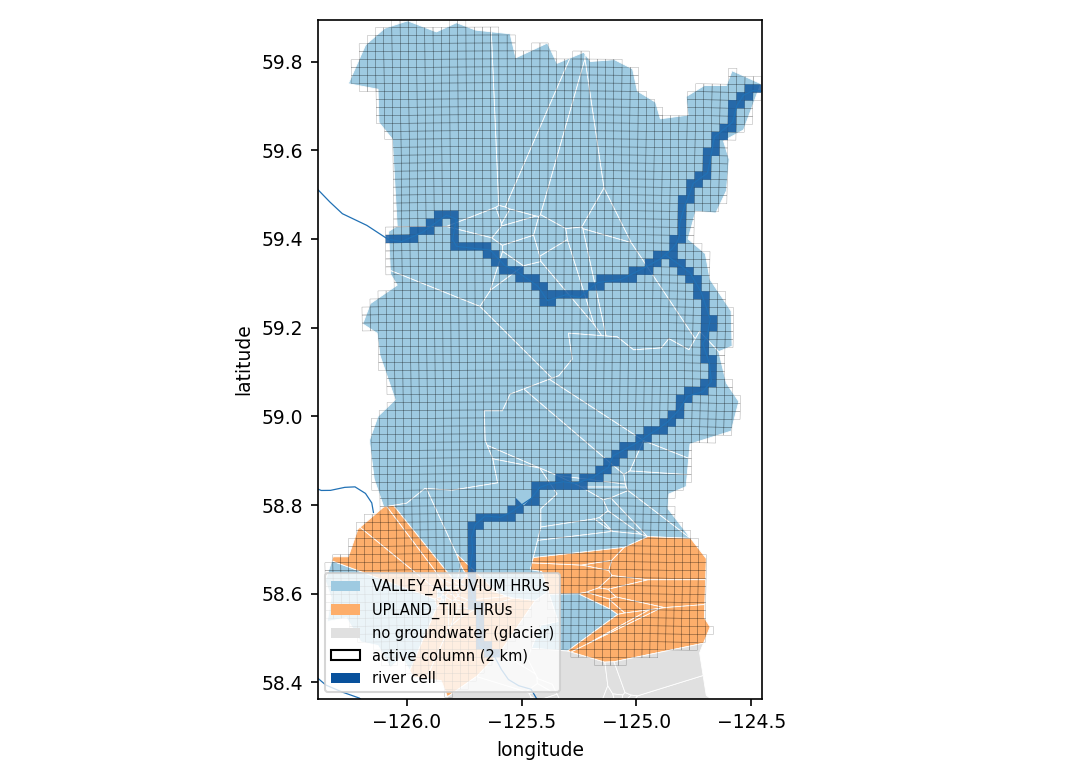
\includegraphics[width=0.9\linewidth]{figures/fig_grid_liard.png}
\caption{Example~A: coupled HRUs (colour = aquifer profile), active 2~km columns and river cells.}\label{fig:ugrid}
\end{figure}

\section{Step 6: look at the results}
\begin{itemize}
\item \cmd{GWModelSummary.txt}: check the grid, the number of active cells, and that every coupled HRU is linked.
\item \cmd{GWBudget.csv}: the daily groundwater balance (Figure~\ref{fig:budget}). The error column should stay tiny.
\item \cmd{GWHRUState.csv}: the depth to water under each HRU. Figure~\ref{fig:wtdepth} shows the map from
\cmd{mf6/gwf.hds}.
\item \cmd{Hydrographs.csv}: streamflow includes groundwater discharge (Figure~\ref{fig:hydro}).
\end{itemize}
\begin{figure}[!htbp]\centering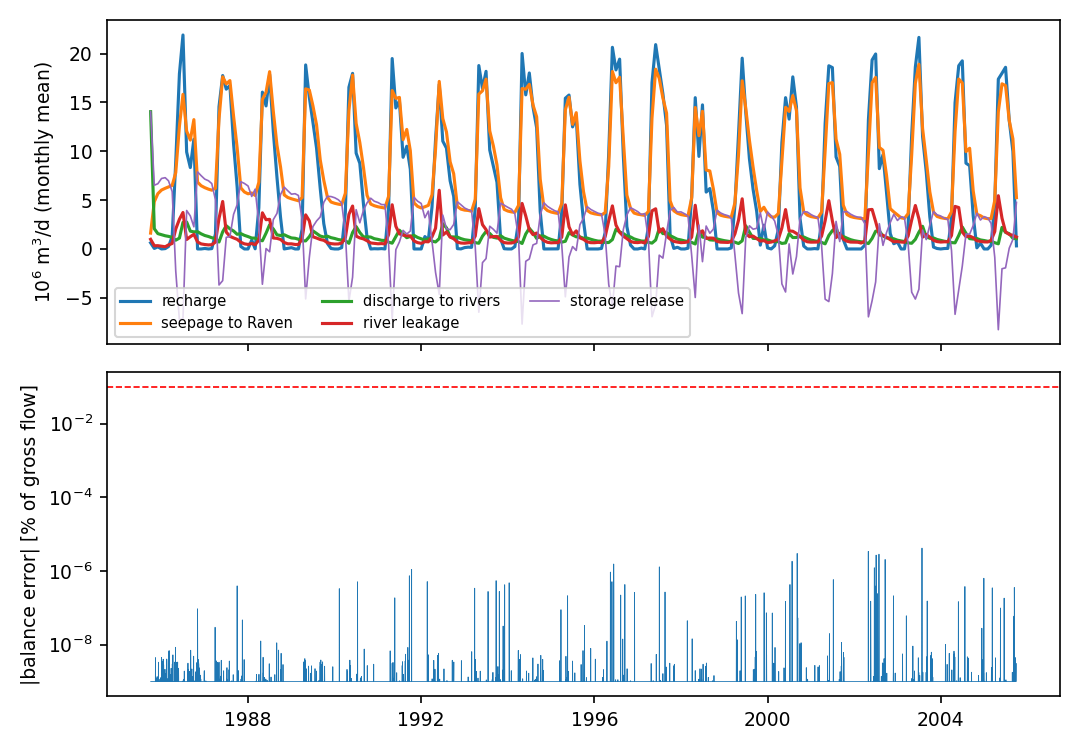
\includegraphics[width=\linewidth]{figures/fig_budget.png}
\caption{Groundwater budget of the 20-year Liard run (monthly means) and daily balance error; the dashed line is 0.1\%.}\label{fig:budget}\end{figure}
\begin{figure}[!htbp]\centering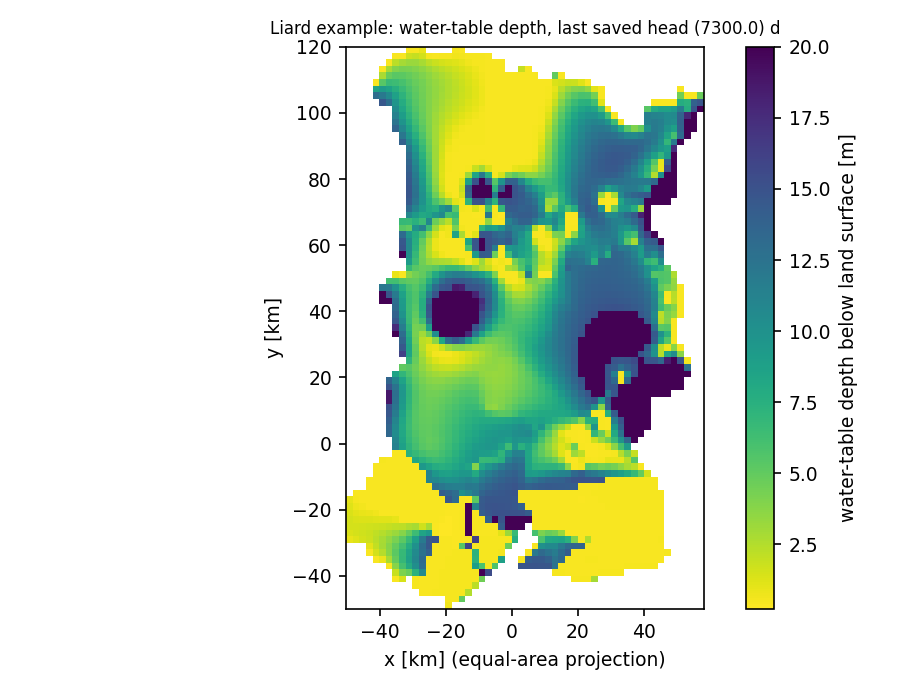
\includegraphics[width=0.72\linewidth]{figures/fig_wtdepth.png}
\caption{Depth to water at the last saved head.}\label{fig:wtdepth}\end{figure}
\begin{figure}[!htbp]\centering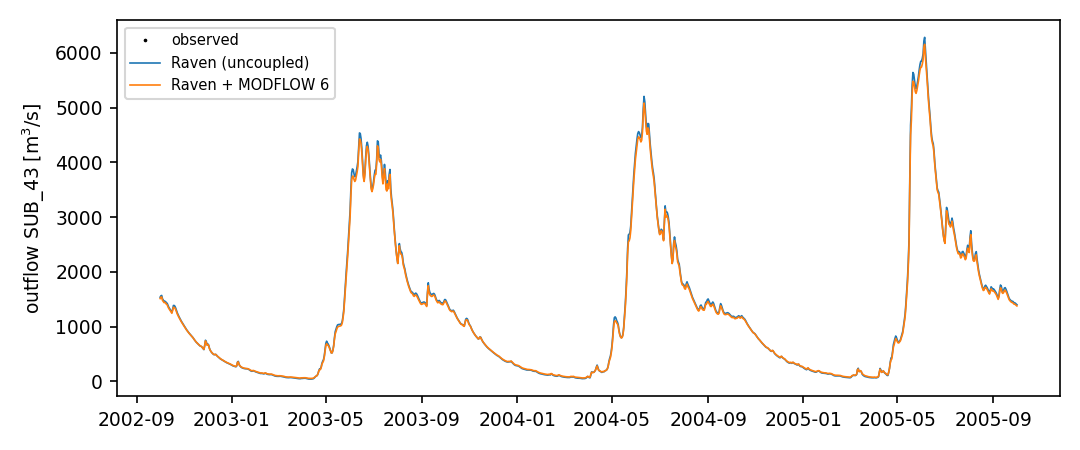
\includegraphics[width=\linewidth]{figures/fig_hydrograph.png}
\caption{Outflow of subbasin 43, 2003--2005, without and with groundwater (not recalibrated).}\label{fig:hydro}\end{figure}
Without recalibration and with stand-in geometry, the Nash--Sutcliffe efficiency at gauges 10BE004, 10BE005 and 10BE010
changes from 0.867, 0.835, 0.681 to 0.850, 0.821, 0.634. Recalibrating with flow and head data is the natural next step
(Chapter~\ref{uch:restarts}). Chapter~\ref{uch:outputs} explains every output and how to check the water balance.
